% !TEX root = ../main_hessenberg.tex
%\section{Loopless digraphs and examples}\label{sec:loopless}

We now show that loopless digraphs correspond to subsets $S$ avoiding both
endpoints and consecutive elements, and their count is governed by Fibonacci
numbers.

%\subsection{Loop characterization}

\begin{lemma}[\leanlink{HessenbergDigraphs.lean}{L117-L132}{loop\_iff\_mem\_R\_and\_C} \leanlink{HessenbergDigraphs.lean}{L133-L147}{loop\_at\_one} \leanlink{HessenbergDigraphs.lean}{L148-L164}{loop\_at\_n} \leanlink{HessenbergDigraphs.lean}{L165-L177}{loop\_at\_mid}]\label{lem:loops-in-model}
Let $n \ge 2$ and $S \subseteq [n-1]$. The digraph $D_n(S)$ has a loop at
vertex $v$ if and only if $v \in R \cap C$. Equivalently:
\begin{itemize}[leftmargin=2em]
\item $1 \to 1$ is an arc if and only if $1 \in S$;
\item $n \to n$ is an arc if and only if $n - 1 \in S$;
\item for $2 \le v \le n - 1$: $v \to v$ is an arc if and only if
  $\{v - 1, v\} \subseteq S$.
\end{itemize}
\end{lemma}
\begin{proof}
A loop $(v, v)$ is an overlay arc (spine arcs have $i = j + 1 \neq j$), so it
exists if and only if $v \in R$ and $v \in C$. Substituting the definitions
$R = \{1\} \cup \{k + 1 : k \in S\}$ and $C = S \cup \{n\}$ yields the three
cases.
\end{proof}

\begin{corollary}[\leanlink{HessenbergDigraphs.lean}{L194-L225}{loopless\_iff}]\label{cor:loopless-characterization}
A connected support digraph $D(Q)$ is loopless if and only if
$D(Q) = D_n(S)$ for a subset $S \subseteq \{2, \dots, n-2\}$ containing no
two consecutive elements.
\end{corollary}
\begin{proof}
By Lemma~\ref{lem:loops-in-model}, absence of loops at $1$ and $n$ forces
$1 \notin S$ and $n - 1 \notin S$, i.e., $S \subseteq \{2, \dots, n-2\}$.
Absence of loops at interior vertices $v \in \{2, \dots, n-1\}$ means that
for no $v$ do we have both $v - 1 \in S$ and $v \in S$; equivalently, $S$
contains no pair of consecutive elements.
\end{proof}

%\subsection{Fibonacci enumeration}

The number of subsets of $\{0, \dots, m-1\}$ containing no two consecutive
elements is well known to be the Fibonacci number $F_{m+2}$. Shifting the
domain to $\{2, \dots, n-2\}$ (size $n - 3$ for $n \ge 3$), we obtain
$F_{n-1}$ loopless active sets. Applying the same isomorphism analysis as in
Theorem~\ref{thm:count} gives:

\begin{theorem}[\leanlink{HessenbergDigraphs.lean}{L1238-L1249}{count\_loopless\_formula}]\label{thm:loopless-nonisomorphic}
Let $n \ge 3$. The number of non-isomorphic loopless connected support digraphs
of real orthogonal upper Hessenberg matrices of size $n$ is
\[
N_n^{\mathrm{loopless}}
= F_{n-1} - \left\lfloor \frac{n-3}{2} \right\rfloor,
\]
where $F_k$ denotes the $k$-th Fibonacci number ($F_0 = 0$, $F_1 = 1$,
$F_{m+2} = F_{m+1} + F_m$).
\end{theorem}
\begin{proof}
By Corollary~\ref{cor:loopless-characterization}, loopless connected digraphs
correspond to subsets $S \subseteq \{2, \dots, n-2\}$ without consecutive
elements; there are $F_{n-1}$ such subsets. As in Theorem~\ref{thm:count},
subsets of size $\ge 2$ are rigid, the empty set yields $1$ class, and the
$n - 3$ singletons partition into $\lceil(n-3)/2\rceil$ classes. The total is
\[
N_n^{\mathrm{loopless}}
= (F_{n-1} - (n-3) - 1) + \lceil(n{-}3)/2\rceil + 1
= F_{n-1} - \lfloor(n{-}3)/2\rfloor. \qedhere
\]
\end{proof}

%\subsection{Examples}

We illustrate the theory with two $5 \times 5$ examples. In each case we display the matrix $Q$, its adjacency matrix $A$, and the resulting digraph.

\begin{example}[$n = 5$, $S = \{2\}$]\label{ex:D5S2}
The parameters $(\alpha_1, \alpha_2, \alpha_3, \alpha_4) = (1, \tfrac{1}{2}, 1, 1)$ yield:
\[
Q = \begin{pmatrix}
0 & \tfrac{1}{\sqrt{2}} & 0 & 0 & \tfrac{1}{\sqrt{2}} \\
-1 & 0 & 0 & 0 & 0 \\
0 & -\tfrac{1}{\sqrt{2}} & 0 & 0 & \tfrac{1}{\sqrt{2}} \\
0 & 0 & -1 & 0 & 0 \\
0 & 0 & 0 & -1 & 0
\end{pmatrix},
\qquad
A = \begin{pmatrix}
0 & 1 & 0 & 0 & 1 \\
1 & 0 & 0 & 0 & 0 \\
0 & 1 & 0 & 0 & 1 \\
0 & 0 & 1 & 0 & 0 \\
0 & 0 & 0 & 1 & 0
\end{pmatrix}.
\]
The Hamilton cycle is $1 \to 5 \to 4 \to 3 \to 2 \to 1$. Since
$R = \{1, 3\}$ and $C = \{2, 5\}$ are disjoint, the digraph is loopless
(Figure~\ref{fig:D5S2}).
\end{example}

\begin{figure}[htbp]
\centering
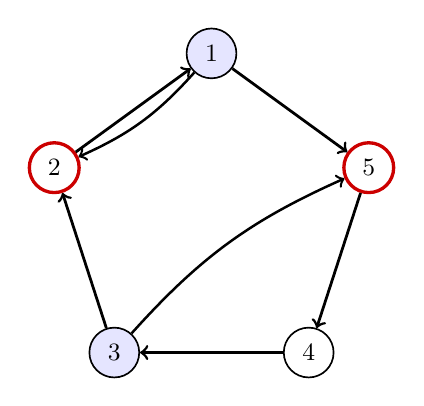
\begin{tikzpicture}[
  v/.style={circle, draw=black, line width=0.6pt, inner sep=1.2pt,
            minimum size=18pt, font=\small},
  cyc/.style={->, line width=1.0pt, draw=black},
  extra/.style={->, line width=0.9pt, draw=black},
  Rnode/.style={fill=blue!10},
  Cnode/.style={draw=red!80!black, line width=1.2pt}
]
\node[v,Rnode] (1) at ( 90:2.1) {1};
\node[v,Cnode] (5) at ( 18:2.1) {5};
\node[v]       (4) at (-54:2.1) {4};
\node[v,Rnode] (3) at (-126:2.1) {3};
\node[v,Cnode] (2) at (162:2.1) {2};

\draw[cyc] (1) -- (5);
\draw[cyc] (5) -- (4);
\draw[cyc] (4) -- (3);
\draw[cyc] (3) -- (2);
\draw[cyc] (2) -- (1);

\draw[extra, bend left=12] (1) to (2);
\draw[extra, bend left=12] (3) to (5);
\end{tikzpicture}
\caption{The loopless support digraph $D_5(\{2\})$. Active rows $R = \{1,3\}$
(blue fill) and active columns $C = \{2,5\}$ (red outline) are disjoint.}
\label{fig:D5S2}
\end{figure}

\begin{example}[$n = 5$, $S = \{1, 3\}$]\label{ex:D5S13}
The parameters $(\alpha_1, \alpha_2, \alpha_3, \alpha_4) = (\tfrac{1}{2}, 1, \tfrac{1}{2}, 1)$ give:
\[
Q = \begin{pmatrix}
\tfrac{1}{\sqrt{2}} & 0 & \tfrac{1}{2} & 0 & \tfrac{1}{2} \\
-\tfrac{1}{\sqrt{2}} & 0 & \tfrac{1}{2} & 0 & \tfrac{1}{2} \\
0 & -1 & 0 & 0 & 0 \\
0 & 0 & -\tfrac{1}{\sqrt{2}} & 0 & \tfrac{1}{\sqrt{2}} \\
0 & 0 & 0 & -1 & 0
\end{pmatrix},
\qquad
A = \begin{pmatrix}
1 & 0 & 1 & 0 & 1 \\
1 & 0 & 1 & 0 & 1 \\
0 & 1 & 0 & 0 & 0 \\
0 & 0 & 1 & 0 & 1 \\
0 & 0 & 0 & 1 & 0
\end{pmatrix}.
\]
Here $R \cap C = \{1\}$, so there is exactly one self-loop at vertex~$1$
(Figure~\ref{fig:D5S13}).
\end{example}

\begin{figure}[htbp]
\centering
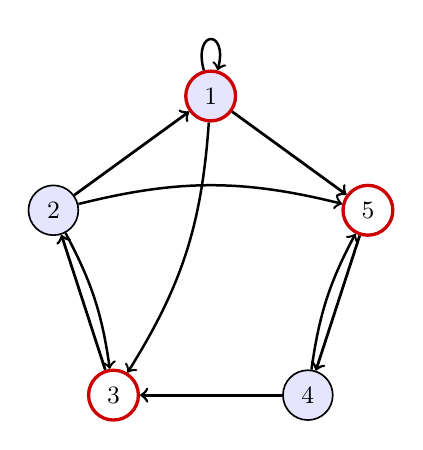
\begin{tikzpicture}[
  v/.style={circle, draw=black, line width=0.6pt, inner sep=1.2pt,
            minimum size=18pt, font=\small},
  cyc/.style={->, line width=1.0pt, draw=black},
  extra/.style={->, line width=0.9pt, draw=black},
  Rnode/.style={fill=blue!10},
  Cnode/.style={draw=red!80!black, line width=1.2pt},
  RCnode/.style={fill=blue!10, draw=red!80!black, line width=1.2pt}
]
\node[v,RCnode] (1) at ( 90:2.1) {1};
\node[v,Cnode]  (5) at ( 18:2.1) {5};
\node[v,Rnode]  (4) at (-54:2.1) {4};
\node[v,Cnode]  (3) at (-126:2.1) {3};
\node[v,Rnode]  (2) at (162:2.1) {2};

\draw[cyc] (1) -- (5);
\draw[cyc] (5) -- (4);
\draw[cyc] (4) -- (3);
\draw[cyc] (3) -- (2);
\draw[cyc] (2) -- (1);

\draw[extra, loop above] (1) to (1);
\draw[extra, bend left=14] (1) to (3);
\draw[extra, bend left=10] (2) to (3);
\draw[extra, bend left=14] (2) to (5);
\draw[extra, bend left=10] (4) to (5);
\end{tikzpicture}
\caption{The support digraph $D_5(\{1,3\})$. Since $R \cap C = \{1\}$, there
is exactly one self-loop at vertex~$1$.}
\label{fig:D5S13}
\end{figure}
